\documentclass[10pt, a4paper, twoside, titlepage]{report}

\usepackage[T1]{fontenc}

\usepackage{polski}
\usepackage[utf8]{inputenc}
\usepackage[polish]{babel}
\usepackage[below]{placeins}

\usepackage{amsmath} 
\usepackage{mathtools}
\usepackage[margin=1 in]{geometry}
\usepackage{hyperref}
\usepackage{listings}
%zarzadza wcięciami paragrafów
\usepackage{parskip}
%silne pozycjonowanie obrazow
\usepackage{float}
\usepackage{graphicx}

\newcommand{\textunderbrace}[2]{%
	\ensuremath{\underbrace{\small{\text{#1}}}_{\text{#2}}}%
}
\newcommand{\textoverbrace}[2]{%
	\ensuremath{\overbrace{\text{#1}}^{\text{#2}}}%
}
\renewcommand*\thesection{\arabic{section}}

\newcommand{\stext}[1]{%		
		\begin{lstlisting}
			zawartość...
		\end{lstlisting}
		#1
	}%
    %set title spacing
%\titlespacing*\section{0pt}{12pt plus 4pt minus 2pt}{2pt plus 2pt minus 2pt}
%\titlespacing*\subsection{0pt}{12pt plus 4pt minus 2pt}{2pt plus 2pt minus 2pt}

% font size could be 10pt (default), 11pt or 12 pt
% paper size coulde be letterpaper (default), legalpaper, executivepaper,
% a4paper, a5paper or b5paper
% side coulde be oneside (default) or twoside 
% columns coulde be onecolumn (default) or twocolumn
% graphics coulde be final (default) or draft 
%
% titlepage coulde be notitlepage (default) or titlepage which 
% makes an extra page for title 
% 
% paper alignment coulde be portrait (default) or landscape 
%
% equations coulde be 
%   default number of the equation on the rigth and equation centered 
%   leqno number on the left and equation centered 
%   fleqn number on the rigth and  equation on the left side
%	
\title{Realizacja prostego silnika reguł walidacyjnych przy użyciu technik NLP}
\author{Mariusz Wójcik
}

\date{\today} 
% \date{\today} date coulde be today 
% \date{25.12.00} or be a certain date
% \date{ } or there is no date 
\begin{document}
	% Hint: \title{what ever}, \author{who care} and \date{when ever} could stand 
	% before or after the \begin{document} command 
	% BUT the \maketitle command MUST come AFTER the \begin{document} command! 
	\maketitle
	
	
	\begin{abstract}
	Dokument stanowi raport z realizacji projektu, którego celem było opracowanie metody skutecznego  wykorzystania technik NLP do transkrypcji reguł walidacyjnych zapisanych językiem naturalnym na kod wykonywalny aplikacji.
	
	Dokument składa się z trzech części:
	\begin{enumerate}
		\item Przygotowanie i trening modelu - skupia się ona na zagadnieniach związanych z przygotowaniem próbki uczącej użytej do treningu modelu. 
		\item Aplikacja - część ta dotyczy prezentacji wyników w oparciu o napisaną w tym celu aplikację. 
		\item Ocena wyników - część ta zawiera wykaz problemów, które ujawniłý się podczas pracy nad aplikacją i które nie znalazły należytego rozwiązania.
	\end{enumerate}
	\end{abstract}
	
	%\tableofcontents % create a table of contens 
	
	\tableofcontents
	
   \noindent	
	\part{Przygotowanie i trening modelu}
	\section{Początki}
Jakiś czas temu miałem okazję obejrzeć film, który zrobił na mnie ogromne wrażenie. ,,Arrival - Nowy Początek'' w reżyserii Denisa Villeneuve’a - to obraz niezwykły.
Porusza on problematykę szerokopojętej, wielopłaszczyznowej komunikacji (a czasem skutków jej braku) . W niesamowicie sugestywny i obrazowy sposób pokazuje mechanizm kształtowania się podstaw wspólnego języka i nawiązywania kontaktu.
Proces stopniowego budowania uwspólnionych modeli pojęciowych prowadzący do porozumiewania się tym samym językiem wydał mi się tak logiczny i uporządkowany, że sprawiał wrażenie niemal algorytmicznego...
Pamiętam swoją myśl, że skoro możliwe jest tak precyzyjne określenie
reguł stojących u podstaw nawiązania skutecznej komunikacji, to droga do zbudowania inteligentnych maszyn porozumiewających się z nami ,,ludzkim''
językiem wydaje się już bardzo krótka.

\paragraph{}
Do niedawna wydawało mi się, że porozumiewanie się językiem naturalnym jest domeną przynależną wyłącznie człowiekowi.
Miałem poczucie, że prace nad komputerowym przetwarzaniem języka naturalnego mają wymiar wyłącznie akademicki.
Okazało się jednak, że dynamiczny rozwój algorytmów sztucznej inteligencji i
przetwarzania maszynowego dotknął również tej dziedziny. Gdzieś na styku matematyki, informatyki i lingwistyki wykształciła się
dziedzina, która funkcjonuje jako NLP (ang.  natural language processing ).
	
\paragraph{}
Techniki NLP koncentrują się na analizie, przekształcaniu i generowaniu języka naturalnego.
Dzięki nim komputery nabywają umiejętności nie tylko analizy tekstu, ale również nauki i wyciągania wniosków.
Dają one możliwość analizy nie tylko składni zdań, ale również doszukiwania się ich znaczeń i ukrytych pomiędzy słowami intencji.
Czasami uświadamiam sobie że to wszystko razem brzmi jak czysta fantastyka. Bo jak niby sens, znaczenie i intencje można przeliczyć na liczby i twardo
zakotwiczyć w dziedzinie algebry liniowej ?
\paragraph{}
Tajemnicy tej uchyla jedna z najciekawszych książek, jaką miałem przyjemność ostatnio czytać, mianowicie ,,Natural Language Processing in Action''.
Jest to bardzo przystępnie napisany przewodnik, dzięki któremu łatwiej oswoić się z podstawowymi prawami rządzącymi światem NLP.
Pozycja nie traktuje o rzeczach najłatwiejszych, a mimo to czyta się ją z dużą przyjemnością.
\paragraph{}
Z teorią często jest tak, że w którymś momencie chciałoby się ją zobaczyć w praktyce. Z tej potrzeby zrodził się pomysł na aplikację, którą możnaby
zrealizować przy użyciu technik i algorytmów NLP.
\newline
Przyszedł mi do głowy generator kodu aplikacji, który byłby w stanie przekształcić tekst napisany językiem zbliżonym do naturalnego bezpośrednio do kodu wykonywalnego.  Oczywiście zakładam że tego typu rozwiązanie miałoby zastosowanie do jakiegoś ściśle określonego aspektu działającej aplikacji, np. walidacji dokumentu, czy sprawdzania reguł poprawności modelu dziedziny.  
\newline
I tak właśnie powstał mój miniprojekt, którego celem jest zobaczenie o co tak naprawdę chodzi z tym NLP . :) . Zapraszam do zapoznania się z założeniami i otrzymanymi wynikami.
\paragraph{}
Mam świadomość, że jeśli chodzi o NLP, jestem na początku drogi. Nie mogę powiedzieć nawet tego, że udało mi się zrobić jeden krok, ale wiem jedno...
podróż zapowiada się naprawdę imponująco...
	\section{Założenia i sposób realizacji}
	\section{Abstrakcyjny model reguły}

Przygotowanie próbki rozpocznę od opracowania schematu reguły. 


Na początek wypiszę sobie kilka przykładowych reguł walidacyjnych.
\\ \\
\fbox{\begin{minipage}{40em}
		
		\begin{enumerate}
		\item Jeśli wiek\_pacjenta jest większy od 18 wtedy zgłoś błąd ,,Pacjent jest osobą dorosłą.'', w przeciwnym wypadku
		wyświetl komunikat ,,Pacjent został zakwalifikowany do leczenia pediatrycznego.''.
		\item Jeśli data\_kwalifikacji jest jest mniejsza od '01-01-2019' wtedy zgłoś wyjątek ,,Data sprzed roku 2019.'', w przeciwnym wypadku sprawdź regułę RS-001. 
		\item Gdy saldo\_rachunku jest większe od 100 oraz saldo\_rachunku jest mniejsze niż 1000 wtedy wyświetl komunikat ,,Saldo rachunku jest prawidłowe.'', w przeciwnym razie zgłoś błąd ,,Nieprawidłowe saldo rachunku''.
		\item Jeśli data\_teraz jest niewiększa niż data\_ważności wyświetl komunikat ,,Wniosek jest aktualny.'' w przeciwnym wypadku zgłaszaj błąd ,,Wniosek utracił ważność''.
	\end{enumerate}
	
\end{minipage}}
\\ \\

%\textunderbrace{Ala ma kota}{warunek}
%\textunderbrace{Text \textoverbrace{text}{aaa} text text}{bbb}

%\bigskip

%\emph{\textunderbrace{Text \textoverbrace{text}{aaa} text text}{bbb}}

%tesr\newline\\

Przyjmuję uproszczenie, że każda rozpoznawana reguła składała się będzie z trzech wyróżnialnych bloków:
\\ \\
\fbox{\begin{minipage}{40em}
\[
\underbrace{WARUNKI}  \underbrace{AKCJA\_TAK}  \underbrace{(AKCJA\_NIE)?}
\]
%S\label{fig:test}test
\end{minipage}}
\\ \\

Poszczególne bloki oddzielone będą od siebie słowami kluczowymi oznaczającymi rozpoczęcie i zakończenie bloku. \\

W celu ich wyróżnienia wprowadzam następujące oznaczenia:
\begin{enumerate}
	\item SK\_SW - Start sekcji warunku
	\item SK\_KW - Koniec sekcji warunku
	\item SK\_SAN - Start sekcji akcji wykonywanej przy niespełnionym warunku
\end{enumerate}
Schemat reguły przyjmuje następującą postać:
\\ \\
\fbox{\begin{minipage}{40em}
		\[
		\textunderbrace{SK\_SW}{} \textunderbrace{WARUNKI}{} \textunderbrace{SK\_KW}{} \textunderbrace{AKCJA\_TAK}{}  (\textunderbrace{SK\_SAN}{}\textunderbrace{AKCJA\_NIE)?}{}
		\]
		
\end{minipage}}
\\ \\

Rzut oka na przykład:
\\ \\
\fbox{\begin{minipage}{40em}
			\[
		\textunderbrace{Jeśli}{SK\_SW} 			 
		\]
		\[
		\textunderbrace{data jest mniejsza od '01-01-2019' lub data jest większa niż '01-06-2019'}{WARUNEK} 		 
		\]
		\[
		\textunderbrace{wtedy}{SK\_KW} 		
		\]
		\[ 		
		\textunderbrace{zgłoś wyjątek ,,Data spoza dopuszczonego przedziału.''}{AKCJA\_TAK}		
		\]
			\[		
		\textunderbrace{w przeciwnym wypadku }{SK\_SAN} 	
		\]
		\[			
		\textunderbrace{sprawdź regułę RS-001.}{AKCJA\_NIE} 
		\]
		
\end{minipage}}
\\ \\

\paragraph{}
Ponieważ kluczowe jest właściwe rozpoznanie sekcji warunku, chciałbym wyłączyć go przed nawias i przez chwilę skupić się wyłącznie na nim. 
\\ \\
\fbox{\begin{minipage}{40em}
		
		\[
		\textunderbrace{data jest  mniejsza od '01-01-2019' lub data jest większa niż '01-06-2019'}{WARUNEK} 		 
		\]	
		
\end{minipage}}
\\ \\

Na początek trzeba zauważyć, że powyższa sekcja składa się z dwóch niezależnych wyrażeń warunkowych połączonych operatorem logicznym \textit{lub} . Każdy z pojedynczych warunków składa się z kolei z operatora relacyjnego \textit{(jest mniejsza, jest większa)}, oraz z dwóch operandów \textit{(lewego i prawego)}.
\\
Wprowadzam więc następujące oznaczenia:
\begin{enumerate}
	\item OP\_L - Operand lewy
	\item OPR\_REL - Operator relacyjny
	\item OP\_P - Operand prawy
	\item OPR\_LOG - Operator logiczny
\end{enumerate}

Po podstawieniu, przykładowy warunek można  
\\ \\
\fbox{\begin{minipage}{40em}
		
		\[
		\textunderbrace{\textunderbrace{data}{OP\_L} \textunderbrace{jest  mniejsza od}{OPR\_REL} \textunderbrace{'01-01-2019'}{OP\_P} \textunderbrace{lub}{OPR\_LOG} \textunderbrace{data}{OP\_L} \textunderbrace{jest większa niż}{OPR\_REL} \textunderbrace{'01-06-2019'}{OP\_P}}{WARUNEK} 		 
		\]	
		
\end{minipage}}
\\ \\
Zatem zapis symboliczny sekcji warunkowej będzie wyglądał następująco:
\\ \\
\fbox{\begin{minipage}{40em}
		
		\[
		\textunderbrace{OP\_L OPR\_REL OP\_P (OPR\_LOG OP\_L OPR\_REL OP\_P)?}{WARUNEK} 		 
		\]	
		
\end{minipage}}
\\ \\

Po dokonaniu podstawienia w sekcji \textit{WARUNKI} abstrakcyjny model reguły przyjmie następującą postać:
\\ \\
\fbox{\begin{minipage}{40em}
		\[
		\underbrace{SK\_SW}
		\]
		\[	
			\textunderbrace{OP\_L OPR\_REL OP\_P (OPR\_LOG OP\_L OPR\_REL OP\_P)?}{WARUNEK}		
		\]
		\[
			\underbrace{SK\_KW}
		\]
		\[
		\underbrace{AKCJA\_TAK}
		\]
		\[
		(\underbrace{SK\_SAN}\underbrace{AKCJA\_NIE)?}
		\]
		
\end{minipage}}
\\ \\
Jeśli chodzi o akcje, to sprawa wydaje się prostsza, bo każda z nich składa się z części mówiącej o tym co ma być zrobione (AKCJA), oraz z jakim parametrem ma być wykonane (AKCJA\_PARAMETR). Ostatecznie więc, po wykonaniu podstawienia nasz model przyjmie następującą, ostateczną formę:
\\ \\
\fbox{\begin{minipage}{40em}
	\[
		\underbrace{SK\_SW}
		\]
		\[	
		\textunderbrace{OP\_L OPR\_REL OP\_P (OPR\_LOG OP\_L OPR\_REL OP\_P)?}{WARUNEK}		
		\]
		\[
		\underbrace{SK\_KW}
		\]
		\[
		\textunderbrace{AKCJA AKCJA\_PARAMETR}{AKCJA\_TAK}
		\]
		\[
		(\underbrace{SK\_SAN}\textunderbrace{AKCJA AKCJA\_PARAMETR}{AKCJA\_NIE})?
		\]
		
		\begin{enumerate}
			\item SK\_SW - Start sekcji warunku
			\item SK\_KW - Koniec sekcji warunku
			\item SK\_SAN - Start sekcji akcji wykonywanej przy niespełnionym warunku
				\item OP\_L - Operand lewy
			\item OPR\_REL - Operator relacyjny
			\item OP\_P - Operand prawy
			\item OPR\_LOG - Operator logiczny
		\end{enumerate}
		
\end{minipage}}
\\ \\
I jeszcze ostatnie spojrzenie na przykład:
\\ \\
\fbox{\begin{minipage}{40em}
		\[
		\textunderbrace{Jeśli}{SK\_SW} 			 
		\]
		\[
	\textunderbrace{\textunderbrace{data}{OP\_L} \textunderbrace{jest  mniejsza od}{OPR\_REL} \textunderbrace{'01-01-2019'}{OP\_P} \textunderbrace{lub}{OPR\_LOG} \textunderbrace{data}{OP\_L} \textunderbrace{jest większa niż}{OPR\_REL} \textunderbrace{'01-06-2019'}{OP\_P}}{WARUNEK} 		 
	\]	
		\[
		\textunderbrace{wtedy}{SK\_KW} 		
		\]
		\[ 		
		\textunderbrace{\textunderbrace{zgłoś wyjątek}{AKCJA} \textunderbrace{,,Data spoza dopuszczonego przedziału.''}{AKCJA\_PARAMETR}}{AKCJA\_TAK}		
		\]
		\[		
		\textunderbrace{w przeciwnym wypadku }{SK\_SAN} 	
		\]
		\[			
		\textunderbrace{\textunderbrace{sprawdź regułę}{AKCJA} \textunderbrace{ RS-001.}{AKCJA\_PARAMETR}}{AKCJA\_NIE} 
		\]
		
\end{minipage}}
\\ \\

Tak określony model może być podstawą do wygenerowania odpowiednio oznakowanej próbki uczącej.

	\section{Przygotowanie próbki uczącej}
Mechanizmy NER wchodzące w skład OpenNLP pozwalają na stworzenie własnego modelu i przyuczenie go do rozpoznawania specyficznych bytów domenowych. Próbka ucząca jest dosyć obszernym zbiorem przykładów (dokumentacja OpenNLP mówi o minimum 15 tyś. zdań), w których w specjalny sposób otagowane zostały kluczowe frazy. 
\\ \\
\fbox{\begin{minipage}{40em}
		\small{		
		<START:SK\_SW> jeśli <END> <START:OP\_L> xxx <END> <START:OPR\_REL> jest większy niż <END> <START:OP\_P> xxx <END> <START:SK\_KW> wtedy <END> <START:AKCJA> zgłoś błąd <END> <START:AKCJA\_PARAMETR> xxx <END> . 	
	}			
\end{minipage}}

\paragraph{}
Byty nazwane, które ma rozpoznawać model należy umieścić pomiędzy tagami \\ \textit{<START:NAZWA\_BYTU>} i \textit{<END>}. Każda reguła moich danych uczących jest zbudowana według schematu omawianego wcześniej abstrakcyjnego modelu reguły. Zgodne z nim są również nazwy encji.
W przypadku tych części reguły, które są zmienne i specyficzne dla każdej instancji (takie jak komentarze, nazwy operandów, wszelkie parametry) użyłem frazy \textit{xxx}, która oznacza że będzie tu coś, o czym na tym etapie nie możemy nic powiedzieć (znamy tylko pozycję tego tokena względem innych encji ). 

	\section{Trening modelu}

Proces trenowania modelu realizowany jest przez niewielką aplikację (\textit{Kotlin, OpenNLP NER API}),której zadaniem jest dostarczenie danych próbki, ustawienie parametrów uczenia, wystartowanie procesu trenowania, oraz zapisanie wygenerowanego binarnego pliku modelu. Najistotniejszy fragment aplikacji przedstawiony jest na listingu. 
\small
\begin{lstlisting}
private fun trenujModel(aZbiorRegul:Path): TokenNameFinderModel {
	// reading training data
	var inputFactory: InputStreamFactory?
	try {
		inputFactory =
		 MarkableFileInputStreamFactory(aZbiorRegul.toFile())
		} catch (e: FileNotFoundException) {
			throw IllegalArgumentException(e)
		}

	var sampleStream: ObjectStream<*>?

	sampleStream = NameSampleDataStream(
	PlainTextByLineStream(inputFactory, StandardCharsets.UTF_8))

	// setting the parameters for train ing
	val params = TrainingParameters()
	params.put(TrainingParameters.ITERATIONS_PARAM, 70)
	params.put(TrainingParameters.CUTOFF_PARAM, 1)

	// training the model using TokenNameFinderModel class
	var nameFinderModel: TokenNameFinderModel?
	try {
		nameFinderModel = NameFinderME.train("en"
		, null
		, sampleStream
		,params
		, TokenNameFinderFactory.create(null
					, null
					, mutableMapOf<String, Any>()
					, BioCodec()))

	return nameFinderModel

	} catch (e: IOException) {
		throw IllegalArgumentException(e)
	}
}
\end{lstlisting}
	
\normalsize
Raport podsumowujący pojedynczą sesję treningową wykonaną w oparciu o przygotowaną wcześniej próbkę wygląda następująco:

\small
\begin{lstlisting}

> Task :app-modul-silnik-regul:wytrenujModel
=====encje_reguly_probka_uczaca.reg
Indexing events with TwoPass using cutoff of 1

Computing event counts...  done. 259140 events
Indexing...  done.
Collecting events... Done indexing in 6,59 s.
Incorporating indexed data for training...  
done.
Number of Event Tokens: 259140
Number of Outcomes: 13
Number of Predicates: 654
Computing model parameters...
Performing 70 iterations.
1:  . (259100/259140) 0.9998456432816238
2:  . (259140/259140) 1.0
3:  . (259140/259140) 1.0
4:  . (259140/259140) 1.0
5:  . (259140/259140) 1.0
Stopping: change in training set accuracy less than 1.0E-5
Stats: (259140/259140) 1.0
...done.
Compressed 654 parameters to 322
79 outcome patterns
Trained model saved to file in location=>src/main/resources/modelnlp/encje_reguly_model.bin
\end{lstlisting}
\normalsize
\paragraph{}\noindent
Trening modelu jest krokiem kończącym etap przygotowawczy. Zapisany plik binarny jest gotowy do użycia go w aplikacji. W następnej części postaram się opisać jak można posłużyć się nim do rozwiązania konkretnego problemu.
	\part{Aplikacja}
	\section{Architektura aplikacji}

Aplikacja egzaminująca model składa się z dwóch warstw - części GUI i części serwerowej. Część serwerowa odpowiedzialna jest za całościową analizę reguł, oraz generowanie kodu. Jest ona napisana w technologii Spring Boot, w języku Kotlin. Warstwa GUI stworzona została przy użyciu biblioteki Angular. Komunikacja pomiędzy obydwoma częściami odbywa się przy pomocy serwisów REST. 

Z punktu widzenia użytkownika aplikacja składa się z trzech wyraźnie wyodrębnionych części

\begin{enumerate}
	\item Sekcji danych wejściowych
	\item Sekcji wyników analizy NLP
	\item Sekcji wygenerowanego kodu
\end{enumerate}


\subsection{Sekcja danych wejściowych}
W tej części aplikacji użytkownik może zarządzać danymi, jakie poddawane są analizie NLP. Interfejs aplikacji umożliwia dodawanie nowych reguł, modyfikację treści istniejących, oraz kasowanie reguł. 
\begin{figure}[H]
	\centering
	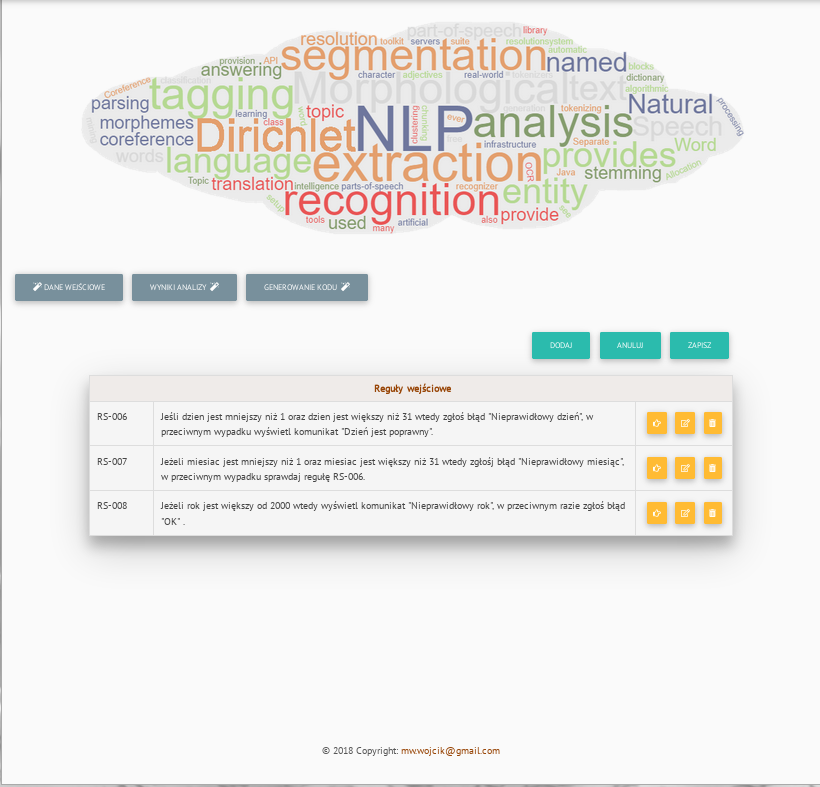
\includegraphics[scale=0.7]{img/app/app-we.png}
	\caption{Główne okno aplikacji - sekcja definicji reguł wejściowych}\label{app-ekran-we}
\end{figure}
\subsection{Sekcja prezentacji wyników analizy NLP}
Ten ekran jest nieco ciekawszy od poprzedniego. Prezentuje wyniki analizy reguł wykonanej w
oparciu o algorytmy uczenia maszynowego dostępne w ramach biblioteki \textit{OpenNLP}.
Wyniki analizy prezentowane są w tabelach według następującego schematu:

\begin{enumerate}
	\item \textbf{Reguła wejściowa} - informacja o treści reguły poddawanej analizie algorytmicznej.
	\item	\textbf{Wyodrębnione komunikaty} - jest to lista komunikatów użytkownika, które zostały odnalezione w regule.W celu uproszczenia przetwarzania sekwencji przez algorytmy NLP komunikaty są wyodrębniane i zastępowane
	słowem - markerem identyfikującym komunikat. Jako komunikat uznaje się ciąg znaków otoczonych znakiem podwójnego cudzysłowu.
	\item \textbf{Rozpoznane tokeny}-jest to tabela pokazująca wyniki działania algorytmu NLP. Prezentuje ona regułę rozbitą na pojedyncze tokeny.
	Przy każdym tokenie  wskazana jest logiczna encja, do której przyporządkował go algorytm dokonujący analizy, oraz liczbowe prawdopodobieństwo z jaką nastąpiło dopasowanie.
	Ostatnia kolumna tej tabeli ma zastosowanie tylko do wybranych bytów logicznych i służy do normalizacji tokenów. Np. tokeny "równy", "równa", "jest równy" należą do jednej wspólnej kategorii oznaczającej równość "==", a tokeny "jest większy lub równy", "jest nie mniejszy niż" oznaczają kategorię ">="
	\item \textbf{Rozpoznane parametry wejściowe}- w tabeli tej prezentowane są tokeny uznane jako parametry wejściowe do reguły. Zwykle występują one w wyrażeniach warunkowych.
	W przypadku gdy warunek reguły skonstruowany jest w taki sposób, że następuje porównanie z wartością stałą (np liczbową lub datę), wtedy taka wartość jest traktowana jako parametr wejściowy reguły z przypisaną wartością domyślną.
	Warunkiem poprawności analizy reguły jest właściwe przyporządkowanie typów danych do parametrów reguły. Jeśli nie uda się wnioskowanie automatyczne, to informacje te muszą być wprowadzone przez użytkownika w do drugiej kolumny tabeli parametrów.
	\item \textbf{Rozpoznane wywołania innych reguł}-W tabeli tej prezentowane są odnalezione odwołania do innych reguł,oraz mapowania parametrów wejściowych reguły wołającej i reguły wołanej.
\end{enumerate}
\paragraph
Prezentacja wyników następuje po wybraniu reguły z listy w panelu bocznym. Zielony znacznik świadczy o tym że dopełnione zostały wszystkie doprecyzowania i mapowania parametrów, więc aplikacja posiada komplet informacji potrzebnych do wygenerowania kodu.


\begin{figure}[H]
	\centering
	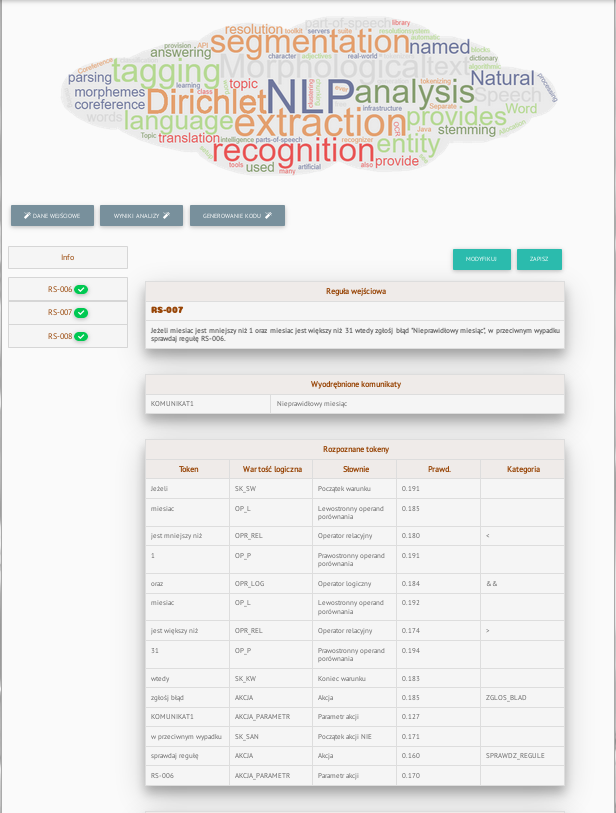
\includegraphics[scale=0.7]{img/app/app-reg.png}
	\caption{Główne okno aplikacji - sekcja analizy NLP}\label{app-ekran-wyniki}
\end{figure}

\subsection{Sekcja wygenerowanego kodu}
W trzeciej sekcji programu pokazany jest wynik przekształcenia reguły do kompilowalnego kodu \textit{Kotlin}. Dla każdej reguły tworzona jest osobna metoda. Nazwa metody jest tożsama z kodem reguły. Metoda przyjmuje parametry, które zaprezentowane są w tabeli ,,Parametry wejściowe'' na ekranie wyników analizy. 
\begin{figure}[H]
	\centering
	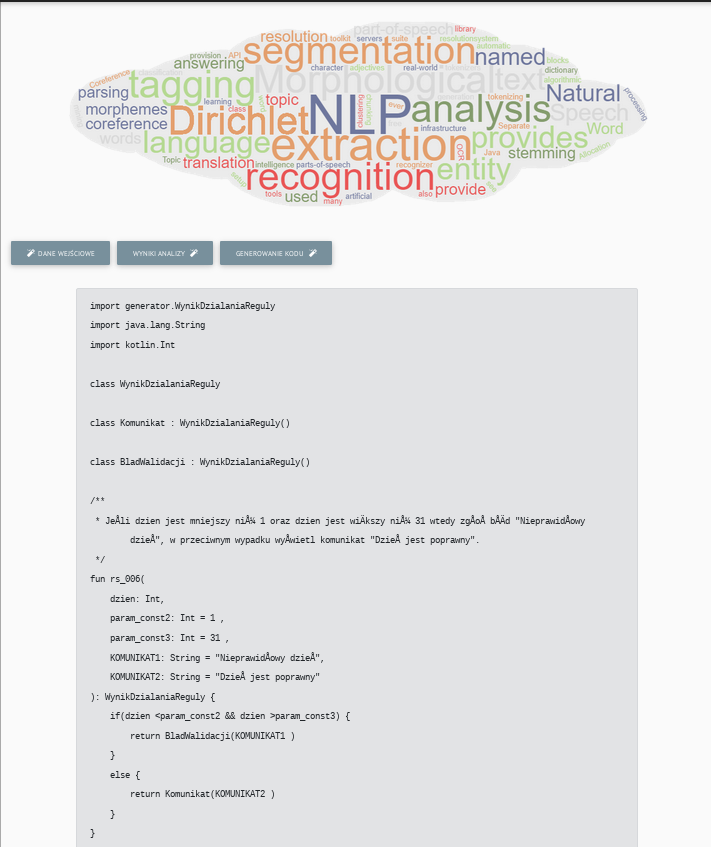
\includegraphics[scale=0.7]{img/app/app-kod.png}
	\caption{Główne okno aplikacji - sekcja wygenerowanego kodu}\label{app-ekran-kod}
\end{figure}

Uwaga! Sekcja ta jest dostępna tylko wtedy, gdy wszystkie reguły zaprezentowane na ekranie analizy danych \ref{app-ekran-wyniki} zostaną zwalidowane pozytywnie, czyli aplikacja uzyska wszystkie dane potrzebne do wygenerowania kodu.
	\section{Eksperymenty}
Teraz chciałbym pokazać jak działa moja aplikacja. W tym celu spróbuję trochę poeksperymentować z danymi i pokazać to, co do tej pory udało się osiągnąć.

\subsection{Reguła z jednym warunkiem i jedną akcją}
Wyobraźmy sobie sytuację że robimy system rejestrujący badania medyczne wykonane na rzecz pacjenta. Chcielibyśmy się dowiedzieć, czy rejestrowane badanie jest badaniem refundowanym (nasza wyobrażona refundacja dotyczy tylko badań zarejestrowanych w roku 2019). O czasie rejestracji badania mówi zmienna ,,data\_rejestracji\_badania''. W przypadku gdy badanie nie jest refundowane system ma wyświetlić komunikat informacyjny. 

Na początek definicja reguły, niech brzmi ona następująco:
\\ \\
\fbox{\begin{minipage}{40em}
\textit{Jeżeli data\_rejestracji\_badania jest mniejsza niż '01-01-2019' wtedy wyświetl komunikat "Badanie sprzed okresu refundacji".}
\end{minipage}}
\\ \\
Wprowadzam ją do systemu, i wygląda to tak:
\begin{figure}[H]
	\centering
	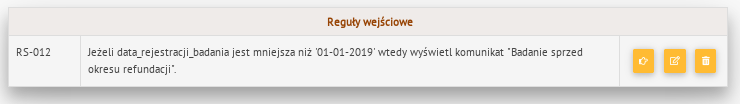
\includegraphics[scale=0.8]{img/app-eksperymenty/p1-1.png}
\end{figure}

\newpage
Teraz spójrzmy czego udało się o niej dowiedzieć:
\begin{figure}[H]
	\centering
	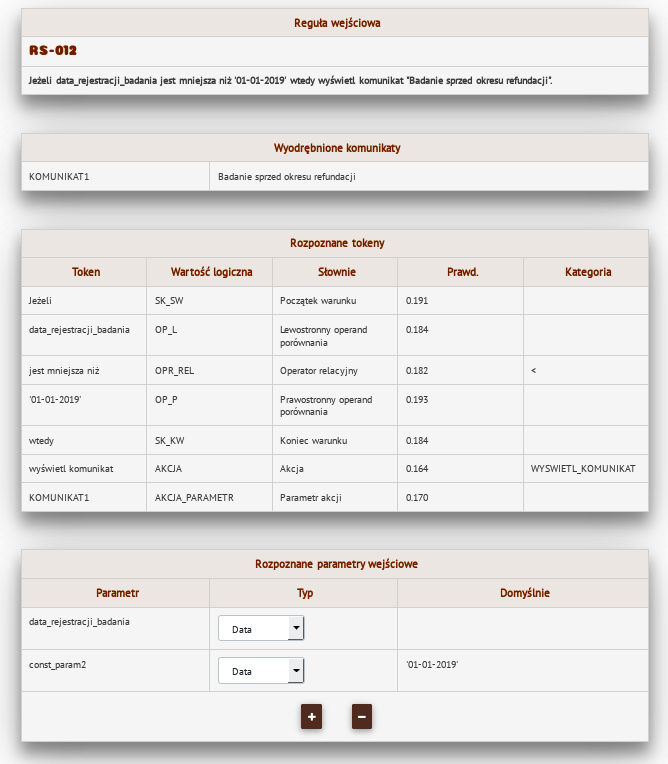
\includegraphics[scale=0.9]{img/app-eksperymenty/p1-2.png}
\end{figure}

\begin{itemize}
	\item \textbf{Reguła wejściowa} - system jeszcze raz przypomina treść wprowadzonej reguły i prezentuje nadany jej kod, w naszym przypadku RS-012.
	\item \textbf{Wyodrębnione komunikaty} - tu zaprezentowane zostały komunikaty, które udało się wyszukać w regule. Każdy odnaleziony komunikat zostaje wycięty z reguły przed poddaniem jej analizie i zastąpiony swoim reprezentującym go identyfikatorem - w naszym przypadku odnaleziony został jeden komunikat i zastąpiony przez słowo \textit{,,KOMUNIKAT1''}.
	\item \textbf{Rozpoznane tokeny} - najistotniejsza część wyników analizy. Widzimy, że z tą regułą algorytm poradził sobie bezbłędnie. Tokeny zostały prawidłowo skojarzone z ich znaczeniem logicznym. \\
	Na chwilę uwagi zasługuje tylko kolumna ,,Kategoria'' . Dotyczy ona tych tokenów, które mogą być określone na wiele sposobów. Musimy przyporządkować im jedną, uniwersalną kategorię. Jako przykład niech posłuży operator mniejszości - może on zostać opisany jako (,,jest mniejszy niż'',,,jest mniejszy od'',,,jest mniejsza od'',\dots). Z punktu widzenia aplikacji, wszystkie te wartości reprezentują jedną kategorią, ja nazwałem ją po prostu ,,<'' .
	\item {Rozpoznane parametry wejściowe} - w tym miejscu pokazywane są wartości, które uznane zostały za parametry wejściowe reguły. Trafiają tu tokeny, które biorą udział w porównaniach, lub są przekazywane jako parametry wejściowe do innych reguł (tę sytuację pokażę trochę później). W tym przypadku widzimy, że aplikacji udało się prawidłowo dopasować typy danych i określić wartość domyślną jednego z parametrów. Gdyby to się nie udało, czynność tę musi wykonać człowiek. Musi się to stać przed wygenerowaniem kodu.
\end{itemize}


I na koniec spójrzmy na wygenerowany kod metody walidującej regułę RS-012.
\begin{figure}[H]
	\centering
	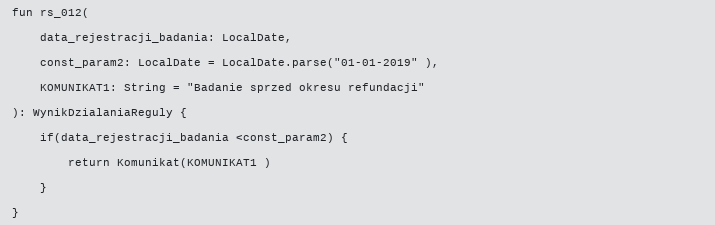
\includegraphics[scale=0.8]{img/app-eksperymenty/p1-3.png}
\end{figure}

Wszystko wygląda ok, więc spróbujmy trochę skomplikować regułę. 

\subsection{Reguła z podwójnym warunkiem}
Załóżmy że refundacji podlegają tylko te badania, które zostały wykonane w pierwszym kwartale 2019 roku. Chcielibyśmy zmienić treść reguły w taki sposób, by po stwierdzeniu tego typu sytuacji informowała użytkownika że jego badanie może zostać zrefundowane.
\\ \\
\fbox{\begin{minipage}{40em}
		\textit{Jeżeli data\_rejestracji\_badania jest mniejsza niż '01-01-2019' lub data\_rejestracji\_badania nie jest większa niż '01-04-2019' wtedy wyświetl komunikat "Badanie sprzed okresu refundacji".}
\end{minipage}}
\\ \\
Modyfikuję regułę:
\begin{figure}[H]
	\centering
	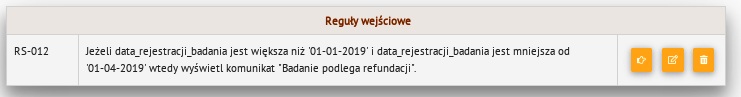
\includegraphics[scale=0.8]{img/app-eksperymenty/p2-1.png}
\end{figure}
I oglądamy wyniki:
\begin{figure}[H]
	\centering
	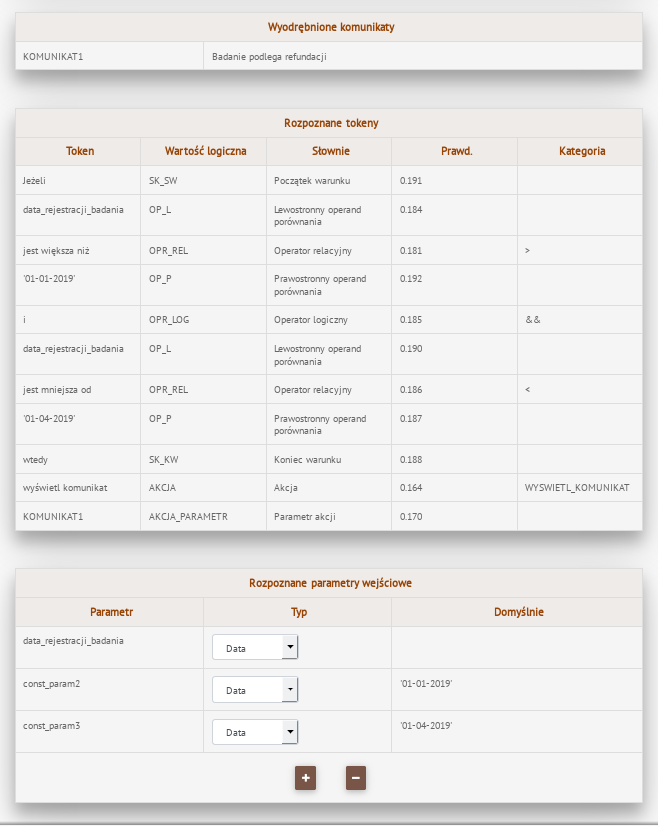
\includegraphics[scale=0.8]{img/app-eksperymenty/p2-2.png}
\end{figure}
Istotne zmiany doszły w tabeli rozpoznanych tokenów. Doszedł operator logiczny, oraz druga część warunku. Udało się również prawidłowo przyporządkować operatory do określających je kategorii. Dodatkowo pojawił się nowy parametr wejściowy, który definiuje drugą z porównywanych wartości. 

Wygenerowany kod również wygląda na poprawny:
\begin{figure}[H]
	\centering
	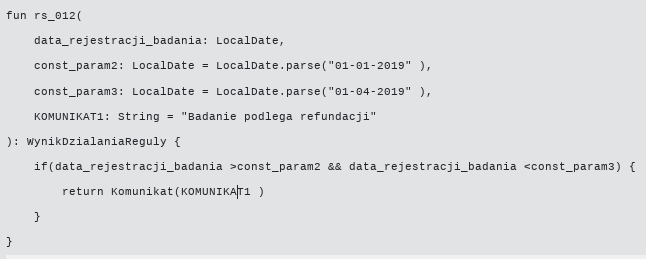
\includegraphics[scale=0.8]{img/app-eksperymenty/p2-3.png}
\end{figure}

\subsection{Reguła z akcją ,,w przeciwnym wypadku''}
Załóżmy, że chcielibyśmy by  w przypadku spełnienia warunku reguła wyświetlała stosowny komunikat informacyjny, a w przypadku gdy warunek nie zostanie spełniony zwracała błąd walidacji . \\
Niech będzie ona miała następującą postać:
\\ \\
\fbox{\begin{minipage}{40em}
		\textit{Jeżeli data\_rejestracji\_badania jest większa niż '01-01-2019' i data\_rejestracji\_badania jest mniejsza od '01-04-2019' wtedy wyświetl komunikat "Badanie podlega refundacji", w przeciwnym wypadku zgłoś błąd "Badanie nie może zostać zarejestrowane" .}
\end{minipage}}
\\ \\
Tak jak poprzednio, dokonuję zmian w treści reguły:
\begin{figure}[H]
	\centering
	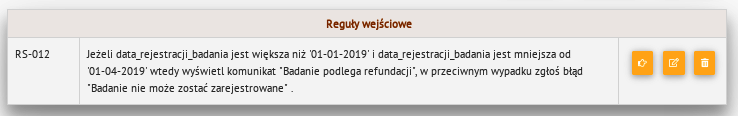
\includegraphics[scale=0.8]{img/app-eksperymenty/p3-1.png}
\end{figure}

W tabeli rozpoznanych tokenów znowu pojawiły się nowe rekordy. Tym razem doszła sekcja związana z akcją ,,NIE''. Wygląda na to, że algorytm poradził sobie również z tą regułą i prawidłowo określił znaczenie poszczególnych słów.

\begin{figure}[H]
	\centering
	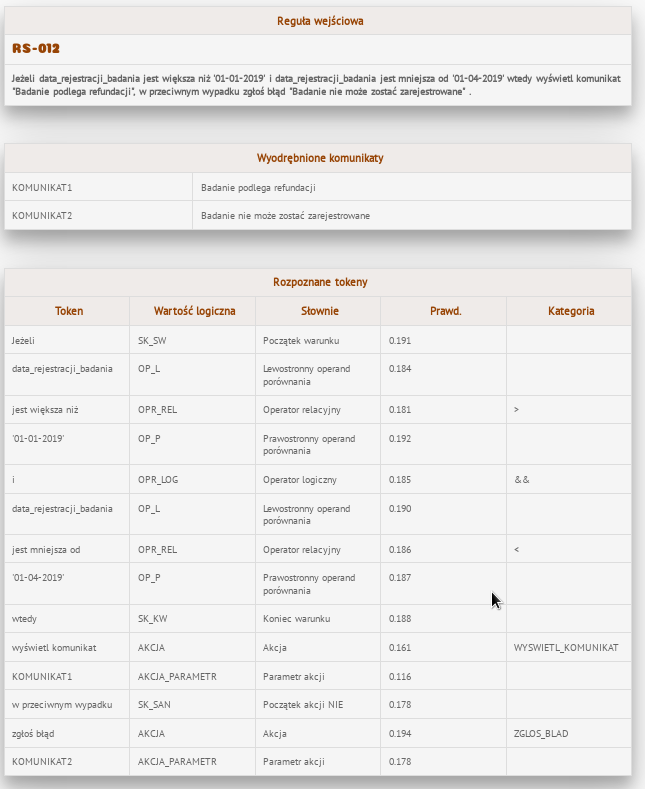
\includegraphics[scale=0.8]{img/app-eksperymenty/p3-2.png}
\end{figure}
Zmiany zaszły również w wygenerowanym kodzie. Nasza instrukcja warunkowa otrzymała część ,,ELSE'', a metoda zwraca nowy typ obiektu.
\begin{figure}[H]
	\centering
	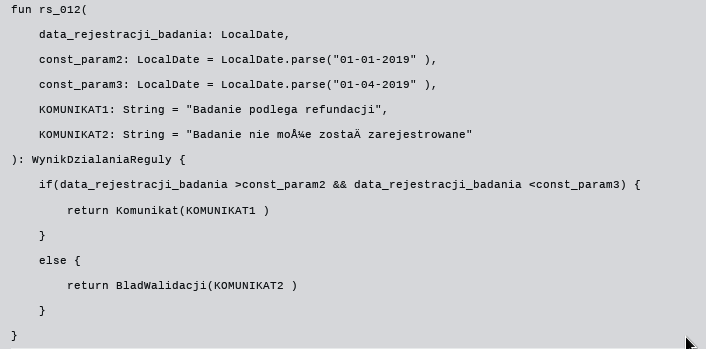
\includegraphics[scale=0.8]{img/app-eksperymenty/p3-3.png}
\end{figure}

\subsection{Reguła z wywołaniem innej reguły}
W tym scenariuszu założymy, że sprawdzanie warunków dat refundacji badania ma obdyć się tylko wtedy, gdy spełniony zostanie warunek odpowiedniego wieku pacjenta. Żeby go zrealizować definiuję nową regułę o następującej treści:
\\ \\
\fbox{\begin{minipage}{40em}
		\textit{dy wiek\_pacjenta jest większy od 18 wtedy zgłoś wyjątek "Przekroczony wiek refundacji", w przeciwnym wypadku sprawdzaj regułę RS-012 .}
\end{minipage}}
\\ \\

\begin{figure}[H]
	\centering
	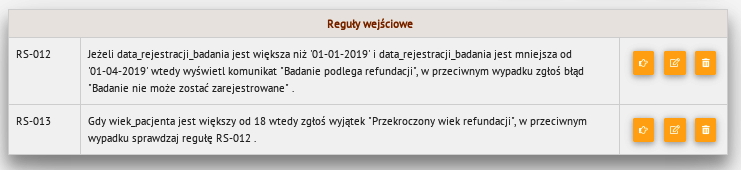
\includegraphics[scale=0.8]{img/app-eksperymenty/p4-1.png}
\end{figure}
Po przejściu do sekcji analizy wyników od razu można zauważyć że pojawiły się nam błędy walidacji  i niemożliwe jest poprawne wygenerowanie kodu.
\begin{figure}[H]
	\centering
	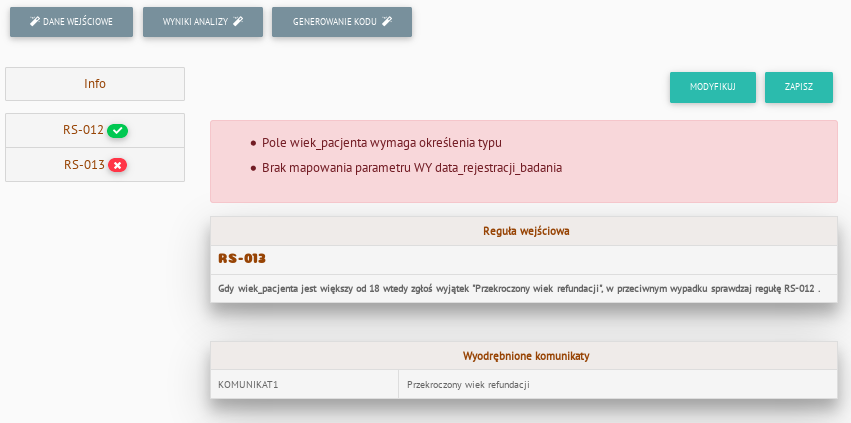
\includegraphics[scale=0.7]{img/app-eksperymenty/p4-1_5.png}
\end{figure}
W sekcji tokenów wszystko wygląda w porządku. Warunki, słowa kluczowe oraz akcje rozpoznane zostały poprawnie.  

\begin{figure}[H]
	\centering
	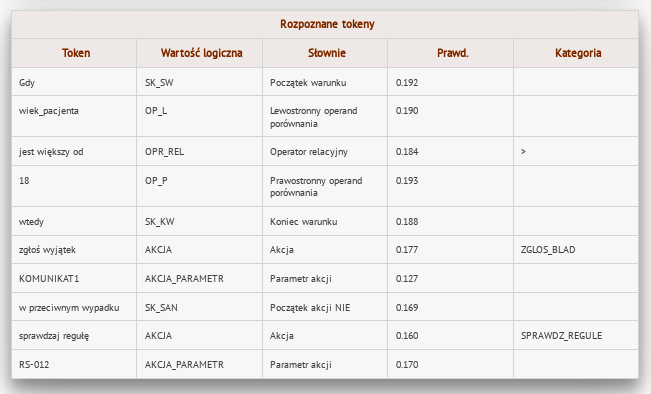
\includegraphics[scale=0.8]{img/app-eksperymenty/p4-2.png}
\end{figure}

Pierwszy problem napotykamy w sekcji ,,Parametrów wejściowych''. Aplikacja prawidłowo rozpoznała zmienną ,,wiek\_pacjenta'' jako parametr, ale z treści reguły nie da się wywnioskować jakiego on jest typu. Wymagana jest pomoc użytkownika. Z listy rozwijanej należy wybrać opcję ,,Liczba''. To załatwia temat pierszego z błędów.
\begin{figure}[H]
	\centering
	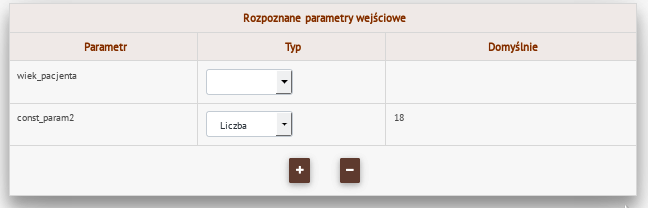
\includegraphics[scale=0.8]{img/app-eksperymenty/p4-3.png}
\end{figure}

Kolejny problem dotyczy samego wywołania reguły ,,RS-012''. Reguła ta na wejściu oczekuje podania daty. W tabeli wywołania użytkownik musi zmapować który parametr wejściowy reguły ,,RS-013'' ma zostać przekazany na wejście reguły ,,RS-012''. I tu pojawia się nowy problem, ponieważ reguła ,,RS-013'' tej daty nie przyjmuje. 

\begin{figure}[H]
	\centering
	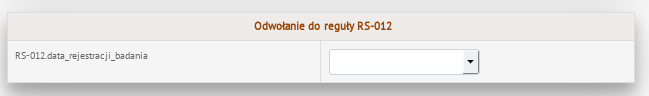
\includegraphics[scale=0.8]{img/app-eksperymenty/p4-4.png}
\end{figure}

Konieczne jest cofnięcie się do tabeli parametrów i użycie opcji dodania nowego parametru - niech nazywa się on ,,data\_badania'' i będzie miał typ ,,Data''. Po tym kroku możliwe staje się wykonanie odpowiedniego przemapowania i po zapisaniu błędy walidacji znikają.
\begin{figure}[H]
	\centering
	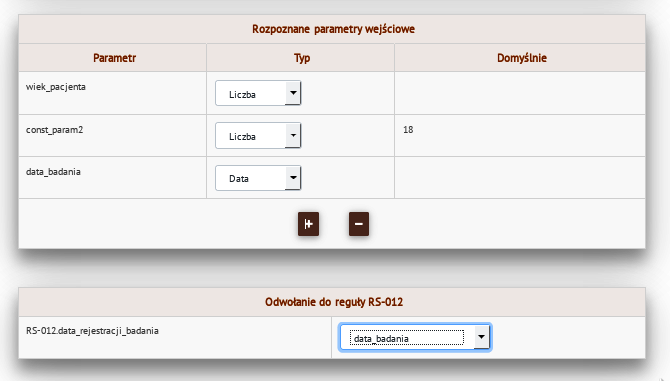
\includegraphics[scale=0.8]{img/app-eksperymenty/p4-5.png}
\end{figure}

Poniżej kod, który teraz już bez przeszkód udało się wygenerować:

\begin{figure}[H]
	\centering
	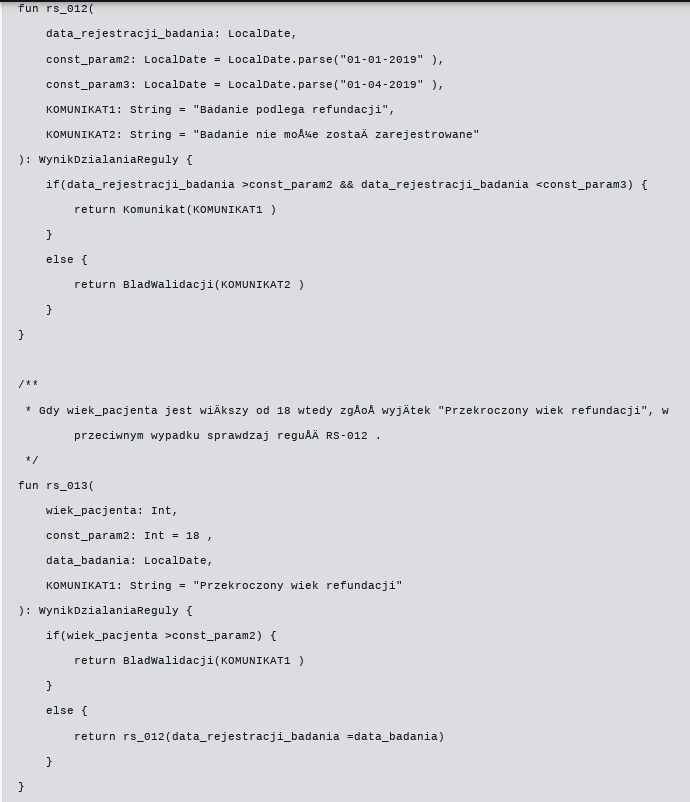
\includegraphics[scale=0.8]{img/app-eksperymenty/p4-6.png}
\end{figure}
	\section{Próbki zaburzone}
Teraz chciałbym jeszcze trochę poeksperymentować z treścią reguł poddawanych analizie i przyjrzeć im się pod kątem odporności na różnego typu zaburzenia takie jak np. literówki czy niepoprawna struktura reguł. 
\subsection{Literówki i nieznane słowa}
Jako oznaczenie akcji, które mają zostać wykonane wprowadzam określenia, które nigdy nie pojawiły się w danych uczących. 
\\ \\
\fbox{\begin{minipage}{40em}
		\textit{Jeżeli data\_rejestracji\_badania jest większa niż '01-01-2019' i data\_rejestracji\_badania jest mniejsza od '01-04-2019' wtedy \textbf{zaprezentuj komunikat} "Badanie podlega refundacji", w przeciwnym wypadku \textbf{wyrzuć błąd} "Badanie nie może zostać zarejestrowane" . }
\end{minipage}}
\\ \\

\begin{figure}[H]
	\centering
	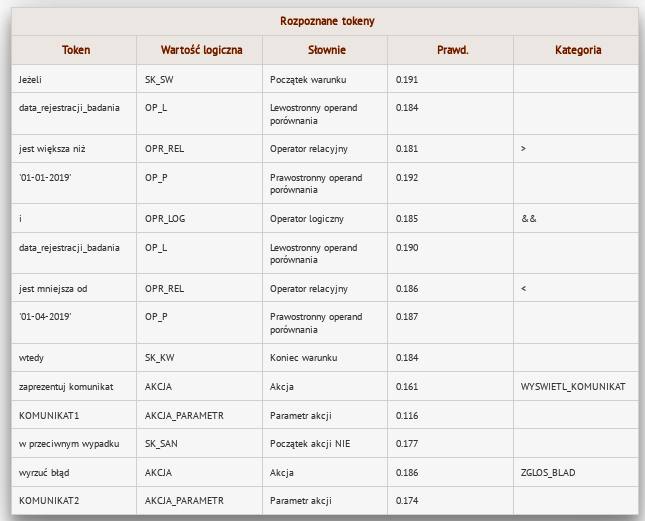
\includegraphics[scale=0.8]{img/app-eksperymenty/p5-1.png}
\end{figure}

Jak widać algorytm znowu sobie poradził,  niestety nie jest to jednak regułą. Tolerancja na błędy pojawia się tylko w niewielkim zakresie. Może jest to związane z niskimi prawdopodobieństwami, z jakimi algorytm rozpoznaje moje encje. 

Dla przykładu wprowadźmy jeszcze jedną modyfikację, tym razem wyrażenie ,,jest mniejsza od'' zamienię na  ,,jest mniejsz od''.
\\ \\
\fbox{\begin{minipage}{40em}
		\textit{Jeżeli data\_rejestracji\_badania jest większa niż '01-01-2019' i data\_rejestracji\_badania \textbf{jest mniejs od} '01-04-2019' wtedy \textbf{zaprezentuj komunikat} "Badanie podlega refundacji", w przeciwnym wypadku \textbf{wyrzuć błąd} "Badanie nie może zostać zarejestrowane" . }
\end{minipage}}
\\ \\

I ta niewielka zmiana wystarczy by algorytm zadziałał źle. Bo chociaż z jednej strony uznał, że fraza ta jest operatorem relacyjnym, to dokonał złej jego kategoryzacji, bo zamiast przypisać go do kategorii ,,<'', trafił on do kategorii ,,>'', niestety z punktu widzenia jakości wygenerowanego kodu, pomyłka ma zasadnicze znaczenie.
\begin{figure}[H]
	\centering
	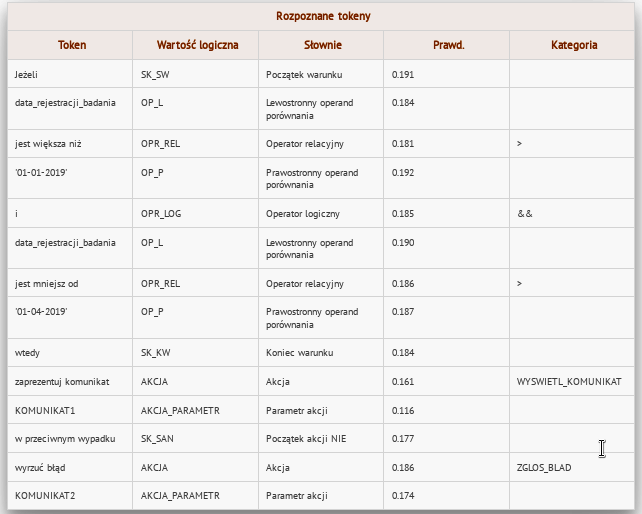
\includegraphics[scale=0.8]{img/app-eksperymenty/p5-2.png}
\end{figure}

\subsection{Zaburzenia struktury i niezgodność z abstrakcyjnym modelem reguły}
Spróbujmy teraz przyjrzeć się reakcji algorytmu na dużo bardziej złożone zaburzenie - niezgodność z przyjetym schematerm reguły. Załóżmy, że z reguły znika słowo ,,WTEDY''.
\\ \\
\fbox{\begin{minipage}{40em}
		\textit{Jeżeli data\_rejestracji\_badania jest większa niż '01-01-2019' i data\_rejestracji\_badania jest mniejsza od '01-04-2019' wyświetl komunikat "Badanie podlega refundacji", w przeciwnym wypadku zgłoś błąd "Badanie nie może zostać zarejestrowane" .}
\end{minipage}}
\\ \\

\begin{figure}[H]
	\centering
	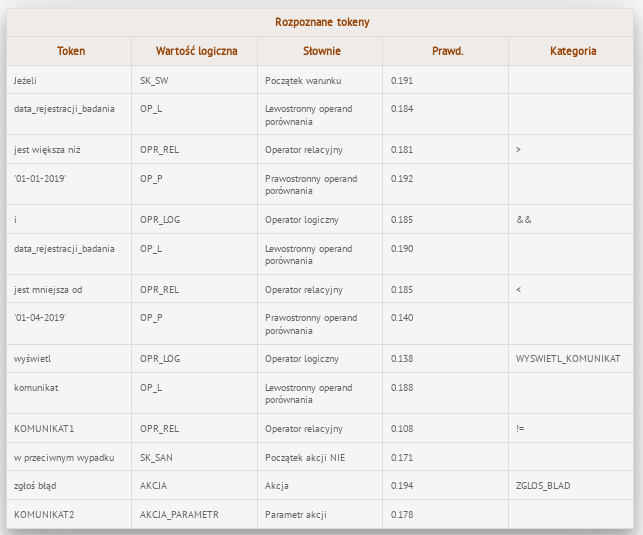
\includegraphics[scale=0.8]{img/app-eksperymenty/p6-1.png}
\end{figure}
Jak można łatwo zauważyć, w tym przypadku algorytm sobie nie poradził. W poszukiwaniu znanego mu wzorca dokonał złych przyporządkowań. Ciekawe natomiast jest to, że mimo pomyłki sekcji rozpoznawania akcji TAK, części reguły leżące poza nią , w sekcji akcji NIE zostały rozpoznane prawidłowo.
\subsection{Podsumowanie}
Niestety w zakresie uodpornienia algorytmu na pomyłki i niezgodności z założoną strukturą pozostało wiele do zrobienia. Stosunkowo niewielkie pomyłki prowadzą do złej interpretacji reguły i wygenerowania wadliwego kodu.
	\part{Ocena wyników}
	\section{Prezentacja wyników}


%	
\section{opis}

	
	\subsection{more introduction}
	Go more in detail \ldots
	
	\subsubsection{even more introduction}
	come to the point \ldots
	
	\paragraph{Paragraphs}
	A paragraph is small but 
	
	\subparagraph{Subparagraphs}
	subparagraphs are smaller! 
	
	\paragraph{Outline}
	First we start with a little example of the article class, which is an 
	important documentclass. But there would be other documentclasses like 
	book \ref{book}, report \ref{report} and letter \ref{letter} which are 
	described in Section \ref{documentclasses}. Finally, Section 
	\ref{conclusions} gives the conclusions.
	
	
	
	\section{Documentclasses} \label{documentclasses}
	
	\begin{itemize}
		\item article
		\item book 
		\item report 
		\item letter 
	\end{itemize}
	
	
	\begin{enumerate}
		\item article
		\item book 
		\item report 
		\item letter 
	\end{enumerate}
	
	\begin{description}
		\item[article\label{article}]{Article is \ldots}
		\item[book\label{book}]{The book class \ldots}
		\item[report\label{report}]{Report gives you \ldots}
		\item[letter\label{letter}]{If you want to write a letter.}
	\end{description}
	
	\section{tabular}
	No paper without a tabular!
	
	\begin{tabular}{|l|c|r|p{2cm}|}
		\hline
		first column & second column & third column & fourth column \\
		\hline 
		l stand for left & c for center & r for right & and p for predefined size \\
		\hline 
	\end{tabular} 
	
	
	\section{some math}
	Math in text is called in line math just put \$ character around 
	the math think. Like $ a^2 + b^2 = c^2 $. It looks better if you use 
	this 
	\[a^2 + b^2 = c^2\]
	
	\section{Conclusions}\label{conclusions}
	There is no longer \LaTeX{} example which was written by \cite{doe}.
	
	\begin{thebibliography}{9}
		\bibitem[Doe]{doe} \emph{First and last \LaTeX{} example.},
		John Doe 50 B.C. 
	\end{thebibliography}






	
\end{document}